\section {System Model}
\label{sec:SYS}

\subsection{Network Topology}
We construct an satellite constellation in \ref{fig:TOPOLOGY}, a polar-orbiting LEO constellation consisting of $w$ low earth orbits and $h$ satellites per orbit. It can provide global coverage at 24 hours. The links between any two satellites call inter-satellite links (ISLs). Because the satellites move in opposite directions will lead to a severe doppler shift, we assume there are no cross-seam ISLs. Therefore, every satellite has four interfaces\cite{4ISL} to construct ISLs with other satellites except for the satellites along the counter-rotating seam; two are intra-plane ISLs, formed by the identical orbit and two adjacent satellites; the others are inter-plane ISLs, formed by two satellites in neighbor orbits. If a satellite moves into the polar region, its inter-plane ISL is disconnected temporarily due to the physical limits such as antenna tracking, while the intra-plane ISLs are maintained on all occasions.

\begin{figure}[H]
	\centering
	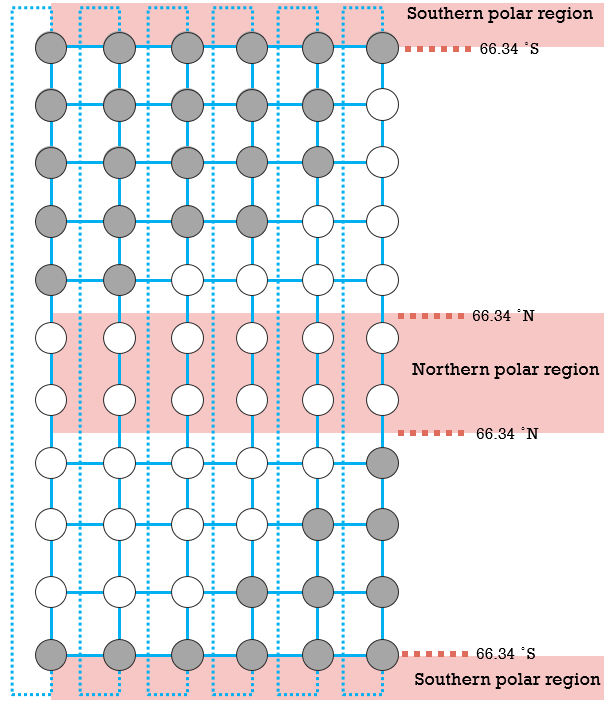
\includegraphics[scale=0.9,clip, width=0.5\textwidth]{fig/Topology.png}	
	\caption{Topology of satellite network}
	\label{fig:TOPOLOGY}
\end{figure}

The satellite network topology is regular because the movements of satellite follow the laws of motion. Then we discretize the continuously changing topology structure into several time intervals $\Delta t =[t_0, t_1], [t_1, t_2],...,[t_{n-1}, t_n]$. The labels will not change in each interval.

The LEO satellite position can be predicted/determined by Two Line Element (TLE). TLE is a data format encoding a list of orbital elements of an Earth-orbiting object for a given point in time and is made publicly by the Joint Space Operations Center(JSpOC). The local satellite can obtain the TLE of the satellites in the constellation from the ground periodically(about 6 hours \cite{TLE}).

The satellites on polar-orbit will occur counter-rotating, which means two satellites move in opposite directions. The mean orbital velocity of a LEO satellite is about 7.8 km/s.  Two satellites move at high speed and in the opposite directions will lead to a severe Doppler shift, called "seam." Communication with cross-seam ISLs is costly. In this paper, we view it as disconnected\cite{COUNTERROTATING}.

\subsection{Traffic Density Model}
The surface of the earth is divided into $j \times 2j$ grids  and calculated the population density of every grid\cite{TRAFFICDENSITY}, shown in \ref{fig:TRAFFICDENSITY}]. Then every grid $g_i$ obtains a density level $\rho_i$ of traffic.

\begin{figure}[H]
	\centering
	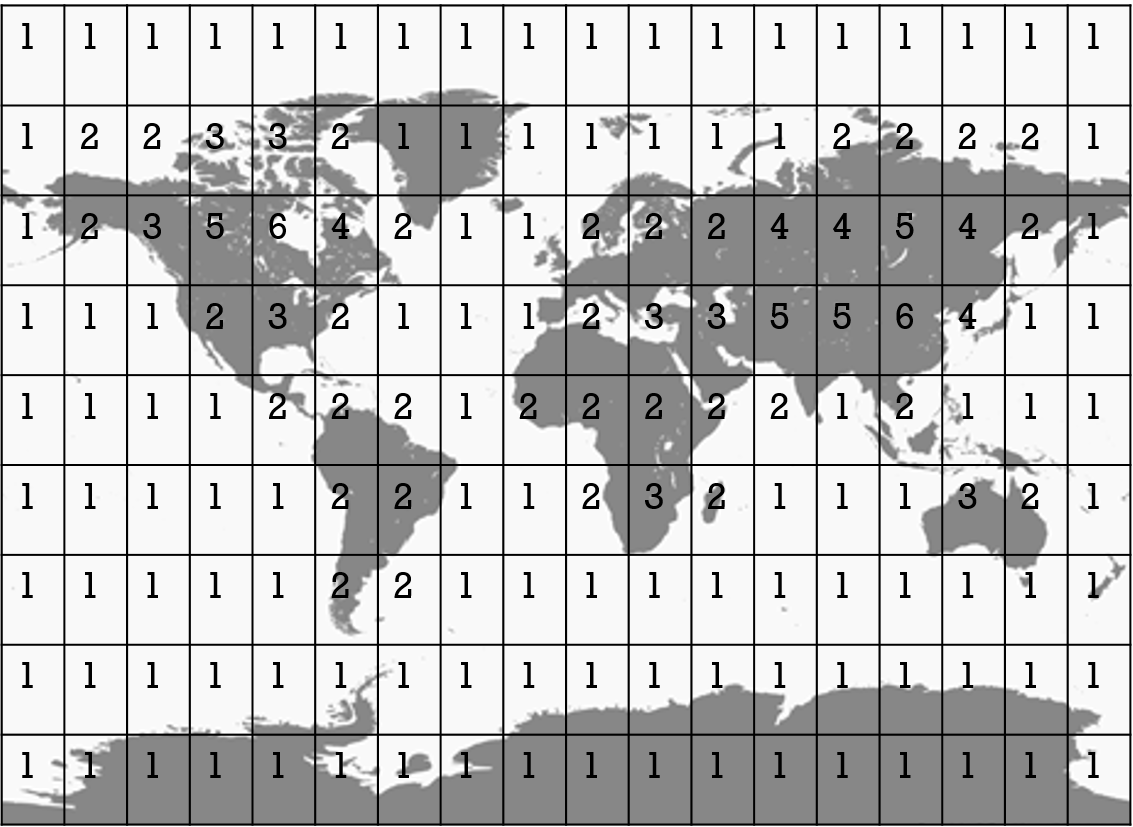
\includegraphics[scale=0.9,clip, width=0.5\textwidth]{fig/TrafficDensity.png}	
	\caption{Density level on grid map}
	\label{fig:TRAFFICDENSITY}
\end{figure}

The density level $\rho$ of each grid is calculated as:
\begin{equation}
 l_{a} \approx \frac{R \pi}{j} \cos \left(\theta_{\text {grid }}\right) 
\end{equation}

\begin{equation}
 l_{b} \approx \frac{R \pi}{j} 
\end{equation}

\begin{equation}
 A \approx l_{a} l_{b}=\left(\frac{R \pi}{j}\right)^{2} \cos \left(\theta_{g r i d}\right) 
\end{equation}

\begin{equation}
 \rho=\frac{N_{u}}{A} 
\end{equation}

where $A$ represents the area of each grid, $\theta_{grid}$ is the center latitude value of each grid, $R$ is the Earth radius, $l_{a}$ and $l_{b}$ corresponding to the length of each grid along the longitude and latitude direction, and $N_u$ is the number of users in the grid. Then each vertical projection of the satellite onto the surface of the Earth can be mapped to one of the grids, and it denoted each satellite has a traffic density level $D_n$.